\chapter{Acknowledgements}
\section{Funding}
This project was funded by a Big Lotteries grant to the Communities Living Sustainably (CLS) group. We are especially thankful for the support provided by CLS and Candida Blaker.
\begin{marginfigure}[2.0 cm]
 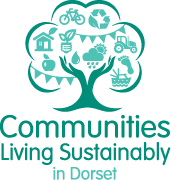
\includegraphics{img/clslogo.png}
 %\caption{Kingston Maurward College, Dorchester}
\end{marginfigure}

\section{Organisation Project Initiation}
Staff at Dorset Public Health, particularly Chris Ricketts, Rebecca Pearce and Rachel Partridge who applied for funding from CLS, shaped and managed the project on behalf of the public health team. Rebecca also provided ongoing project management and a CLS reporting support throughout the project.

\begin{marginfigure}[2.0 cm]
 
\includegraphics{img/phdlogo.jpg}
 %\caption{Kingston Maurward College, Dorchester}
\end{marginfigure}

\section{Statistical Modelling}
This project relied on the translation of published statistical relationships between thermal stress and excess mortality. This work was undertaken by Dr Dave Lemon, Dorset Public Health. Dave also prepared and presented a poster on this topic at the PHE Applied Epidemiology Scientific Meeting, March 2015.
\section{Project Development}
Dr Chris Skelly was responsible for developing the project, preparing workshops for stakeholder engagement and ultimately for writing up the work that was undertaken -- none of which would have been possible without a team effort.